\documentclass{tesis-usach}
% Opciones: propuesta

\usepackage{nameref}

\begin{document}
\baselineskip 23pt
\frontmatter								% Utiliza numeración romana

% ### Cubierta de la tesis ###
\thispagestyle{empty}
\facultad{Facultad}
\departamento{Departamento}
\grado{Grado}

\titulo{Sistema escalable para la detecci\'on de necesidades en escenarios de cat\'astrofe natural}

\autor{Esteban Andrés Abarca Rubio}
\email{esteban.abarca@usach.cl}
\run{17.679.923-4}		% S\'olo necesario en propuesta
\telefono{997529097}		% S\'olo necesario en propuesta
\annoingreso{2010}

\fecha{Domingo}{15}{Mayo}{2016}

\profesorguia{Nicol\'as Hidalgo Castillo}
\profesorcoguia{Erika Rosas Olivos}

\ciudad{Santiago}
\pais{Chile}

\makecubierta


% ### Páginas preliminares de la tesis ###
\pagestyle{fancy}
\renewcommand{\headrulewidth}{0pt}		% Hace que no aparezca la línea horizontal superior al principio de estas páginas
\fancyhead[L]{}
\fancyhead[C]{}
\fancyhead[R]{}

{\setstretch{1.0}						% Interlineado en las páginas preliminares
\makecopyright							% Si es propuesta no se mostrará

% ### Dedicatoria y agredecimientos de la tesis ###
\dedicatoria{
Dedicado a...
}
		% En caso de no querer agregarlos, comente esta línea
\begin{agradecimiento}
Agradezco a
\end{agradecimiento}

\setcounter{page}{1} 
\resumenCastellano{

\textit{Twitter} es una red social que cuenta con millones de usuarios en todo el mundo y, en Chile, alcanza cerca de los 1.700.000 accesos diariamente. Sus usos van desde ser un \textit{microblog} personal hasta la entrega de información o comunicación entre pares. Es por ello que, en épocas de necesidad, como lo es el periodo inmediato luego de la ocurrencia de una catástrofe natural, las personas tienden a publicar sus experiencias dentro de éste servicio.


Teniendo en cuentra lo anterior es que se construyó un sistema, basado en el paradigma de procesamiento de \textit{streams}, capaz de recoger información de manera automática desde \textit{Twitter} — los denominados \textit{tweets} — y procesarlos a fin de detectar si es que un \textit{tweet} corresponde a uno en el que el usuario haga mención alguno de los tipos de necesidad que el sistema es capaz de detectar y, finalmente, hacer uso de la información implícita (contenido del \textit{tweet} o metadatos), para presentar la necesidad como un punto en un mapa geográfico del país, de modo que la información obtenida pueda ser tomada por las autoridades correspondientes para que, de esta forma, facilite el proceso de toma de desiciones en cuanto al envío de ayuda a una determinada área dadas las necesidades expresadas por la población. 

Para lograrlo se hizo uso de programación extrema en conjunto con la metodología KDD para construir una aplicación que haga uso de un clasificador de textos para la detección de necesidades, mediante los cuales se logra ubicar y clasificar correctamente datos obtenidos del terremoto de Concepción ocurrido el 27 de febrero del año 2010. Además se prueba la efectividad del operador detector de ubicación para suplir la carencia de datos de geolocalización en los metadatos de \textit{Twitter}.

Este trabajo se enmarca en el proyecto FONDEF IDeA (Dos etapas) código ID15I10560 en el que participa un equipo de investigación de la universidad.


\vspace*{0.5cm}
\KeywordsES{Programación extrema; KDD; Clasficador; \textit{Twitter}; Detección de necesidades; Geolocalización; \textit{Stream processing}; Clasificador de texto; Redes sociales; Herramienta de apoyo a desastres}
}

\newpage

\resumenIngles{
\textit{Twitter} is a social network that already has millions of users worldwide and, in Chile, reach about of 1.7 millions of accesses daily. Its uses range from being a personal microblog up to information delivery and comunication between peers. It's because of this that in emergencies, such as the inmediate period after a natural catastrophe, people tends to post their experiences on this service.

With this in mind is that is built a system, based on stream processing paradigm, that it's able to get, automatically, information from \textit{Twitter} — as \textit{tweets} — and process it to detect if a user's \textit{tweet} mentions one of the needs that the system can handle and, finally, use the implicit information in the tweet (metadata) and render the need as a geographical position in country's map, thus authority can use the given information and ease the desition making process of sending help to affected areas with the information given by the population.

To achieve these statements previously exposed extreme programming has been used in conjunction with KDD in order to build a text's classifier to detect people's needs. With these two methods was possible to classify and place correctly the data obtained from Concepción's earthquake at February the 27, 2010. It was proved the effectiveness of the proposed location recognizer created to supply the lack of geolocalization data in Twitter's metadata.

This project is within the FONDEF IDeA (Two stages), code: ID15I10560, where a University's research team is working on.

\vspace*{0.5cm}
\KeywordsEN{Extreme programming; KDD; Classifier; Twitter; Detect people's Need; Geolocalization; Stream processing; Text's classification; Social networks; Post-disaster support tool}
}


% ### Índices ###
\tableofcontents							%% Tabla de contenido

\listoftables							%% Indice de tablas
\listoffigures							%% Indice de figuras
\listofalgorithms						%% Indice de algoritmos
\AtBeginEnvironment{algorithmic}{\setstretch{1.5}} % Interlineado de los algoritmos
} % end \setstretch{1.0}

% ### Cuerpo de la tesis ###
\mainmatter								% Reinicia el contador de páginas para partir de 1 y usando números arábicos.

% ### Capítulos de la tesis ###
\chapter{Introducción}
\label{cap:introduccion}

\section{Antecedentes y motivación}
\label{intro:motivacion}

Los desastres naturales en Chile han sido frecuentes en los últimos años. Sólo por mencionar algunos de los más recientes: la erupción del volcán Chaitén (Mayo, 2008), el terremoto en Tocopilla (Noviembre, 2007), el terremoto en Concepción (2010), el incendio de las Torres del Paine (Diciembre, 2011), el incendio en Valparaíso (Abril, 2014), la erupción del volcán Villarrica (Marzo, 2015), los aluviones en el norte (Marzo, 2015), entre otros. Dependiendo de las características de la emergencia, surgen en la población diversos tipos de necesidades: alimentos, agua, luz eléctrica, refugio, rescate o comunicación. Muchas veces éstas pueden no ser detectadas por las autoridades; al menos, no de forma expedita, lo que resulta perjudicial para las personas que intentan sobrellevar, de la mejor manera posible, la crisis cuando se ve involucrada una necesidad básica, como la falta de agua, donde la vida de los afectados puede verse comprometida. El problema anteriormente descrito, no es sólo para las autoridades; \cite{ChatoSurvey}, señalan que el comportamiento humano ante crisis como éstas, no es quedarse esperando por ayuda o huir en pánico, sino de intentar tomar decisiones rápidas en base a la información que conocen. Esto quiere decir que existe gente dispuesta a ayudar, aun siendo ellos mismos los afectados; pero no siempre disponen de la información necesaria para saber hacia dónde apuntar sus esfuerzos. Será útil, dado todo lo anterior, tener algún medio que concentre las necesidades que pueda tener una población dentro del país, para acudir en su auxilio posterior a la ocurrencia de una emergencia catastrófica, como las mencionadas anteriormente.

Los académicos del proyecto FONDEF IDeA de la Universidad de Santiago de Chile, están trabajando en el desarrollo de una plataforma de procesamiento de flujo de datos generados en contextos de desastres; se busca proveer la infraestructura necesaria para la generación de herramientas capaces de apoyar la toma de decisiones en escenarios de desastres. Esta plataforma hace uso de la información generada por los usuarios en redes sociales como fuente de datos. Para realizar la prueba de concepto de la plataforma se planea desarrollar tres aplicaciones base, orientadas a facilitar la coordinación de voluntarios, detección de necesidades y difusión de información de interés.

En particular, para este trabajo, se ataca el problema de la detección de necesidades de la población y servir de apoyo para la construcción de la plataforma de \textit{streaming}, en relación a qué operadores se han de construir y cómo ha de estructurarse el sistema para operar sobre datos nacionales.

\section{Descripción del problema}
\label{intro:problema}

El problema que aborda esta memoria, es el hacer uso de la información generada por la población por medio de \textit{Twitter} para que, en caso de alguna emergencia de carácter nacional, pueda prestarse apoyo en tiempo real a las autoridades encargadas de la toma de decisiones; por ejemplo, dándoles a conocer en qué lugar exactamente se requiere asistir a la población con un determinado tipo de ayuda, según la necesidad que se presente. ¿Cómo detectar y localizar en tiempo real las necesidades expresadas por la población en redes sociales basadas en texto de manera de entregar generar una nueva fuente de datos para mejorar la toma de decisiones?

\section{Solución propuesta}
\label{intro:solucion}

Se propone un sistema capaz de recoger y analizar de manera automática los eventos generados en la red social \textit{Twitter} en tiempo real, de manera que, al ocurrir un escenario de desastre, determine si la publicación expresa una necesidad y, en caso de que así sea, determine su posición geográfica. 

La solución propuesta consta de dos partes: Por una lado la plataforma y lógica de procesamiento capaz de realizar la labor antes mencionada y, por otro, la visualización de estos datos.

Dado que se utiliza \textit{Twitter} para obtener los datos de entrada, los cuales llegan mediante el \textit{stream} producido por la API de esta red social, la plataforma de procesamiento consiste en un sistema de procesamiento de \textit{streams}, construido utilizando el sistema de computación distribuida de Apache, \textit{Storm}, el cual basa su procesamiento en transformar el problema en un grafo donde cada nodo aporta realizando sólo una tarea, pero que pueden existir múltiples instancias de aquel nodo y éstos pueden estar en diferentes máquinas. Así, internamente, la plataforma está compuesta de operadores que discriminan cuándo evento debe ser entregado a la aplicación de visualización para ser mostradas al usuario. Uno de estos operadores permitirá realizar la categorización del texto de entrada por medio un un clasificador bayesiano.

\section{Objetivos y alcance del proyecto}
\label{intro:objetivos}

\subsection{Objetivo general}
	Construir un sistema escalable para la detección de necesidades de la población en tiempo real, para escenarios de desastre natural haciendo uso de \textit{Twitter}.

\subsection{Objetivos específicos}
\begin{enumerate}
\item	Implementar un método encargado de la recolección de tweets generados dentro del territorio nacional haciendo uso de la API pública de Twitter.
\item	Especificar la taxonomía de las necesidades detectadas.
\item	Diseñar e implementar el clasificador de necesidades.
\item	Definir los elementos de procesamiento para la construcción del sistema capaz de trabajar los datos obtenidos a gran escala.
\item	Implementar una arquitectura escalable que soporte la aplicación.
\item	Evaluar la aplicación bajo condiciones de alto tráfico, como es el caso de una emergencia nacional.
\end{enumerate}

\subsection{Alcances}
\label{subsec:alcances}

Se utilizan las publicaciones de \textit{Twitter} para llevar a cabo el procesamiento de la información y no se considera, en el marco de este trabajo, el uso de una red social alternativa, no porque no sea posible, sino que con el motivo de acotar el problema.

Las necesidades que la aplicación detecta no son una lista exhaustiva de las posibles existentes, sino de un subconjunto que se ha considerado más importante en el equipo de trabajo del proyecto. De esta forma se logra acotar el problema reduciendo la cantidad de categorías y permitir una mayor precisión en la clasificación, entendiendo la precisión como la relación de elementos clasificados correctamente sobre el total.

Se considera, para la construcción del clasificador, un subconjunto de un \textit{dataset} compuesto de cuatro millones de \textit{tweets} recogidos durante y posteriormente al terremoto en Concepción el 27 de Febrero del 2010. Éste conjunto de datos ha de ser limpiado previamente pues contiene \textit{tweets} en idiomas diferentes al idioma objetivo de este trabajo.

El sistema sólo trabaja en la detección con \textit{tweets} que estén en español.

La validación se realiza a partir de \textit{datasets} con \textit{tweets} reales, sin embargo los flujos generados son sintéticos y no obtenidos de manera online desde \textit{Twitter}.

\section{Metodologías y herramientas utilizadas}
\label{intro:metodologia}

\subsection{Metodología}
\label{subsec:MetodologiaDetalle}

Para la realización de este trabajo se utilizan dos metodologías, la primera está enfocada a la búsqueda de información en bases de datos para realizar la construcción del clasificador de texto, mientras que la segunda, una metodología de desarrollo de aplicaciones ágil está enfocada en la construcción en sí de las aplicaciones, tanto de la plataforma de procesamiento como de la aplicación de visualización. Ambas son definidas a continuación.

\subsubsection*{Programación Extrema}
\label{subsubsec:XP}

La Programación Extrema (\textit{Extreme Programming}, XP desde ahora en adelante), comenzó como un proyecto el 6 de Marzo de 1996. Es uno de los procesos ágiles más populares y ha sido probado exitosamente en compañias e industrias de todos los tamaños. \cite{XP}.

Su éxito se debe a que hace especial hincapié en la satisfacción del cliente por sobre la entrega de todo lo el software posible.

Aporta cinco formas escenciales para mejorar el proceso de desarrollo de software: comunicación, simplicidad, retroalimentación, respeto y coraje. Se busca en establecer una estrecha comunicación entre el equipo de desarrollo y el cliente apuntanto, paralelamente, a evitar el sobre-diseño y obtener retroalimentación de modo que los cambios puedan realizarse lo antes posible. 

La metodología implementa unas simples reglas de trabajo, las que se dividen en cinco grandes áreas las que se detallarán a continuación.

\begin{enumerate}
\item Planeación:
	\begin{itemize}
	\item Se escriben Historias de usuario. 
	\item Se crea un plan de \textit{releases}.
	\item Se planifican liberaciones pequeñas y frecuentes.
	\item Se divide el proyecto en iteraciones.
	\item Al comienzo de cada iteración se planea cómo será.
	\end{itemize}
\item Manejo:
	\begin{itemize}
	\item Se le da al equipo una área de trabajo.
	\item Se realizan reunione del tipo \textit{stand up meeting} a díario.
	\item Se mide la velocidad del proyecto. 
	\item Se mueven a las personas de sus puestos (para que todo el equipo pueda trabajar en todo).
	\item Se solucionan problemas que instroduzcan quiebres en la metodología.
	\end{itemize}
\item Diseño:
	\begin{itemize}
	\item Simplicidad. El mejor diseño es el más simple.
	\item Se crean \textit{spikes} para reducir el riesgo.
	\item No se agregan funcionalidades antes de tiempo.
	\item Hacer uso de técnicas de \textit{refactoring}, cada vez que sea posible.
	\end{itemize}
\item Implementación:
	\begin{itemize}
	\item El cliente siempre está disponible. 
	\item El código debe ser escrito bajo estándares. 
	\item Se hace uso de \textit{Test Driven Development }(TDD).
	\item Todo el código debe hacerse haciendo uso de \textit{pair programming}.
	\item Sólo una pareja integra código a la vez.
	\item Integración a menudo.
	\item Se cuenta con un equipo dedicado a la integración.
	\item El código es de todos.
	\end{itemize}
\item Prueba:
	\begin{itemize}
	\item Todo el código debe tener pruebas unitarias.
	\item Todas las pruebas deben ser pasadas antes de una liberación.
	\item Cuando se encuentra un \textit{bug}, se crean pruebas.
	\item Los \textit{test} de aceptación se corren a menudo y sus resultados son publicados.
	\end{itemize}
\end{enumerate}

Éstas reglas por sí solas pueden carecer de sentido, pero se apoyan en los \textbf{valores} que la metodología quiere entregar y que fueron mencionadas anteriormente, pero ahora son detalladas:

\begin{itemize}
\item Simplicidad: Se hace lo que se solicitó, pero no más. Ésto maximiza el valor entregado dado una fecha límite. Nuestras metas se alcanzan por medio de pequeños pasos para mitigar errores tan pronto ocurran. Se crea algo de lo que se esté orgullosos y lo se mantiene en el tiempo a costos razonables.
\item Comunicación: Todos somos partes de un equipo y nos comunicamos cara a cara a diario. Se trabaja juntos en todo: desde la toma de requerimientos hasta la implementación. Se crea la mejor solución posible al problema.
\item Retroalimentación: Cada iteración es completada seriamente entregando \textit{software} funcional. Mostraremos nuestro \textit{software} a menudo y prontamente para luego escuchar y aplicar los cambios solicitados. Se habla de nuestro proyecto y se adapta nuestro proceso a el, no al revéz.
\item Respeto: Todos dan y reciben el respeto que merecen como miembros del equipo. Todos contribuyen con valor así sea simple entusiasmo. Los desarrolladores respetan la experiencia del cliente y viceversa. 
\item Coraje: Se dice la verdad sobre el progreso y nuestras estimaciones. No se documentan excusas por si se falla, pues se planea tener éxito. No tenemos porque no trabajamos solos. Nos adaptaremos a los cambio cuando ocurran.
\end{itemize}

El proceso de XP puede puede ser apreciado en la Figura \ref{fig:procesoXP}.

\begin{figure}[H]
	\centering
	\captionsetup{justification=centering}
	\includegraphics[scale=0.6]{images/flowChartXP.png}
	\caption[Diagrama de flujo de Programación Extrema.]{Diagrama de flujo de Programación Extrema.\\Fuente: \cite{XP}}
	\label{fig:procesoXP}
\end{figure}

\subsubsection*{\textit{Knowledge Discovery in Databases} (KDD)}
\label{subsubsec:kdd}

Metodología de trabajo para la búsqueda de información en bases de datos, es definida por \cite{KDDFayyad} como "el proceso no trivial de identificar patrones válidos, nuevos, potencialmente útiles y en ultima instancia comprensible en los datos", surge de la necesidad de manejar grandes volúmenes de datos e involucra simultaneamente varias disciplinas de investigación tales como el aprendizaje automático, la estadística, inteligencia artificial, sistemas de gestión de bases de datos, sistemas de apoyo a la toma de decisiones, entre otras.

Si bien puede variar el usuario, quien es aquel que determina el domino de la aplicación, es decir, cómo se utilizan los datos, el proceso generalmente considera las siguientes etapas:

\begin{enumerate}
\item Selección de datos: Consiste en buscar el objetivo y las herramientas del proceso de minería, identificando los datos que han de ser extraídos, buscando atributos apropiados de entrada y la información de salida para representar la tarea. Esto quiere decir, primero se debe tener en cuenta lo que se sabe, lo que se quiere obtener y cuáles son los datos que nos facilitarán esa información para poder llegar a nuestra meta, antes de comenzar el proceso como tal.
\item Limpieza de datos: En este paso se limpian los atributos sucios, incluyendo datos incompletos, el ruido y datos inconsistentes. Estos datos sucios, en algunos casos, deben ser eliminados, pues pueden contribuir a un análisis inexacto y resultados incorrectos.
\item Integración de datos: Combina datos de múltiples procedencias incluyendo múltiples bases de datos, que pueden tener diferentes contenidos y formatos.
\item Transformación de datos: Consiste en modificaciones sintácticas llevadas a cabo sobre los datos sin que suponga un cambio en la técnica de minería aplicada. Tiene dos caras, por un lado existen ventajas en el sentido de mejorar la interpretación de las reglas descubiertas y reduce el tiempo de ejecución, por el otro puede llevar a la pérdida de información.
\item Reducción de datos: Reducción del tamaño de los datos, encontrando características más significativas dependiendo del objetivo del proceso.
\item Minería de datos: Consiste en la búsqueda de patrones de interés que puedan expresarse como un modelo o dependencia de los datos. Se ha de de especificar un criterio de preferencia para seleccionar un modelo de un conjunto de posibles modelos. Además se ha de especificar la estrategia de búsqueda (algoritmo), a utilizar.
\item Evaluación de los patrones: Se identifican patrones interesantes que representan conocimiento utilizando diferentes técnicas incluyendo análisis estadísticos y lenguajes de consulta.
\item Interpretación de resultados: Consiste en entender resultados de análisis y sus implicaciones y puede llevar a regresar a algunos pasos anteriores.
\end{enumerate}

La representacíón del proceso descrito por la metodología KDD es presentada en la Figura \ref{fig:procesoKDD}.

\begin{figure}[H]
	\centering
	\captionsetup{justification=centering}
	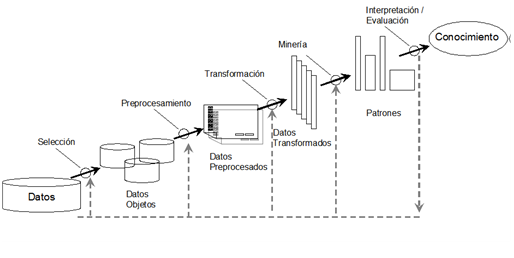
\includegraphics[scale=1]{images/kdd.png}
	\caption[Proceso para el manejo y tratamiento de datos según la metodología KDD.]{Proceso para el manejo y tratamiento de datos según la metodología KDD.\\Fuente: \cite{KDDFigure}}
	\label{fig:procesoKDD}
\end{figure}

\subsection{Herramientas de desarrollo}
\label{subsec:HerrDesarrollo}

A continuación se presentan las herramientas, tanto de \textit{software} como de \textit{hardware} utilizadas para la contrucción del sistema de detección de necesidades.

Se ha se utilizado diversas herramientas de software para la construcción de la aplicación, éstas son descritas a continuación haciendo especial énfasis en aquellas de gran importancia dentro del desarrollo del proyecto

\begin{itemize}
\item Apache Storm: sistema de procesamiento distribuido que basa su procesamiento en dividir el procesamiento en nodos de un grafo dirigido. Permite el procesamiento de eventos en tiempo real.
\item MongoDB: sistema de gestión de bases de datos no-SQL capaz de lidiar con altas tasas de tráfico y respuestas rápidas para aplicaciones en tiempo real.
\item Mallet: biblioteca de Java que contiene herramientas para el procesamiento de lenguaje natural, clasificación de documentos, extracción de información y otras herramientas de aprendizaje automático sobre texto. 
\item Play Framework: \textit{framework} para la contrucción tanto de aplicaciones Java como Scala, utiliza el modelo de arquitectura de diseño modelo-vista-controlador. Está orientado a la construcción de aplicaciones REST y hace hincapié en la productividad de los desarrolladores.
\end{itemize}

Además de las herramientas descritas se hace uso de las una lista de herramientas comunes para el desarrollo de proyectos de \textit{software} presentada a continuación:

\begin{itemize}
\item NetBeans (8.1), como herramienta de apoyo a la construcción de la aplicación.
\item Sublime Text 3 (Build 3103), como editor de textos.
\item MiKTex (XeLaTeX), para la escritura de la memoria.
\item PowerDesigner 16, para la elaboración de diagramas.
\item Bitbucket (Git), como repositorio de todo lo referente al proyecto (detector de necesidades, visualizador y documento de memoria).
\item Windows 10 Home Edition (x64).
\item YourKit 1.8.0\_92 64 bits, para evaluación de \textit{performance} de la aplicación.
\item Linux Mint 17.3 (x86).
\item Oracle VirtualBox (5.0.14).
\end{itemize}

\subsubsection*{Herramientas de \textit{hardware}}
\label{subsubsec:HerrHardw}

Se hace uso del equipo del autor de este trabajo cuyas características técnicas son descritas a contunuación:
\begin{itemize}
\item Procesador Intel Core i5 2.2 Ghz.
\item 8 GB de memoria RAM.
\item 1 TB de disco duro.
\end{itemize}

\section{Organización del documento}
\label{intro:organizacion}

El resto del documento se organiza de la siguiente manera:

El Capítulo \ref{cap:MarcTeorico}, presenta el marco teorico que sustenta la solución implementada y un análisis del estado del arte en términos de las herramientas y tecnicas que han sido utilizadas para dar solucion a problemas similares.

El Capítulo \ref{cap:Requerimientos} describe el proceso de toma de requerimientos de la aplicación. Para ello, siguiendo la metodología XP, se usan de historias de usuario y sus correspondientes criterios de aceptación.

El Capítulo \ref{cap:Diseno}, se presenta la arquitectura del sistema y las decisiones que llevaron a que se se optara por ésta además de describir la implementación de las aplicaciones visualizador y detector de necesidades, incluyendo los elementos que las componen y, en el caso de esta última aplicación, el porqué del uso de una topología en particular.

El Capítulo \ref{cap:experimentos}, describe la completitud de las historias de usuario, evalúa el nivel de replicación de los operadores del sistema y su rendimiento en una simulación de una situación real como fue el terremoto de Concepción en febrero del año 2010.

Finalmente en el Capítulo \ref{cap:conclusiones}, presenta las conclusiones del trabajo realizado, el cumplimiento de objetivos tanto general como específicos, los resultados de los experimentos y trabajo futuro.
\chapter{Marco Teórico}
\label{cap:MarcTeorico}

Este capítulo busca dar a conocer al lector lo último en las áreas que el presente trabajo está inmerso, además de realizar una contextualización de los conceptos necesarios para entender el problema que se está tratando por medio de una breve reseña de cada uno. 

\section{Estado del arte}
\label{intro:motivacion:arte}

Los tópicos que se tratan en esta sección son variados, se comenzará señalando desde donde inicia este trabajo, seguido de las impresiones de distintos autores respecto al trabajo en redes sociales (\textit{Twitter} específicamente), continuando con sistemas de procesamiento para flujos de información para concluir con la construcción de clasificadores para etiquetado de datos.

\subsection{Trabajo previo}
\label{intro:ea:trabajoprevio}

En el marco de las jornadas chilenas de la computación \cite{WladdimiroPMI} propusieron un modelo, desarrollado para el proyecto PMI USA1024, para detectar necesidades de la población ante escenarios de desastres naturales. En se propone un modelo basado en \textit{Yahoo! S4} donde haciendo uso del paradigma de procesamiento de \textit{streams} de datos se forma un grafo cuyos nodos (Elementos de procesamiento o PE, por sus siglas en inglés), dividen el procesamiento en pequeñas tareas fácilmente replicables para paralelizar el \textit{pepeline}. En esa ocación desarrollaron distintos tipos de operadores mencionados a continuación:

\begin{itemize}
\item Recolector: Haciedo uso de la API de \textit{Twitter} obtiene el \textit{stream} de datos del mismo. 
\item \textit{Scheduler}: discrimina cada \textit{tweet} según la categoría que pertenece (Información, agua, electricidad o alimento), mediante el uso de una bolsa de palabras y la distancia \textit{Hamming}.
\item Filtrado: Utiliza un clasificador \textit{Naïve Bayes} para identificar si un \textit{tweet} es subjetivo o no.
\item Relevancia: Identificar si una información es o no confiable haciendo uso de la cantidad de publicaciones del usuario, sus seguidores y a quienes sigue para estimar una reputación del autor.
\item Ranking: Hace uso de la información anterior, decidiendo a qué le entrega mayor importancia.
\end{itemize}

Los autores concluyeron basándose en la carga computacional la importancia de una replicación adecuada para distribuirla entre los PE, pero no fueron concluyentes en cuánto o qué nivel de replicación sería el adecuado o cuándo replicar.

\subsection{La problemática de \textit{Twitter}}
\label{intro:ea:probTwitter}

Diversos autores, entre los que podemos mencionar a \cite{VanDeVoort}, \cite{EventDetectionInTwitter}, \cite{Maldonado}, han señalado las dificultades que se presentan al trabajar utilizando como entradas los estados públicos (\textit{tweet}) de los usuarios de \textit{Twitter}, dentro de las dificultades señaladas se encuentran, por ejemplo, el acceso a la información; si bien existen accesos públicos a la información éstos son restringidos tanto en cantidad como en tiempo: Este punto de acceso permite acceder a un 1\% de la información generada en un instante, es decir, por cada cien \textit{tweets} sólo podra accederse a uno de ellos. Sólo se permite realizar 180 consultas cada quince minutos (aproximadamente 12 consultas por minuto) y, en el caso de ser un usuario identificado, se aumenta a 450 consultas dentro del mismo intervalo de tiempo (aproximadamente 30 consultas por minuto). Por otro lado existe un punto de acceso pagado denominado \textit{FireHose} el cual entrega libre acceso a la información.

Por otro lado \cite{VanDeVoort} señalan que la dificultad radica en el hecho de que cualquier persona puede realizar publicaciones en esta red social, induciendo ruido en la información (considerando el ruido como toda información que aparece junto a la deseada, pero no aporta nueva), además de, al ser publicaciones de máximo 140 caracteres es complejo contextualizar el contenido.

\subsection{Procesamiento de la información}
\label{intro:ea:procesamiento}

Para procesar datos, como los del \textit{stream} de \textit{Twitter}, donde los datos llegan en ráfagas, pueden ser de gran o poco volúmen y requieren de una respuesta inmediata, \cite{HarwoodPeter},hace falta un cambio de paradigma respecto al procesamiento \textit{batch} o procesamiento por lotes, donde un programa ejecuta procesos sin la intervención de terceros desde una base de datos o fichero, por uno donde los datos sean continuos y sin final conocido.
 
Se consideraron tres \textit{frameworks} de computación distribuida: \textit{Apache Storm}, \textit{Apache Spark} y \textit{Apache S4}. El primero presenta una solución basado en el modelo \textit{MapReduce} que toma datos estructurados de la forma (clave, valor) para llevaros a una lista de valores y se usa típicamente para procesar grandes cantidades de datos en distintos nodos que pueden o no estar cercanos físicamente. Los otros dos presentan un modelo basado en el procesamiento de eventos en tiempo real. El problema particular que presenta \textit{S4} es la falta de avances en su desarrollo, el cual ha estado paralizado desde el año 2013. 

\textit{Storm} es un \textit{framework} de computación distribuida para trabajar datos en tiempo real de múltiples fuentes de manera distribuida, tolerante a fallos y de alta disponibilidad. Su funcionamiento se divide en dos elementos: Por un lado existen los \textit{Spout}, encargados de recoger el flujo de entrada de datos, y en segundo, los denominados \textit{bolts}, encajados de procesamiento o transformación de los datos. Por recomendación un \textit{bolt} sólo ha de realizar una tarea. \textit{Storm} puede funcionar de dos formas: En modo \textit{cluster} o modo local; en este último se simula un \textit{thread} por nodo y es utilizado para realizar pruebas locales.

\subsection{Clasificación de textos}
\label{intro:ea:clasificacion}

Por otra parte, la clasificación de texto en servicios de \textit{microblogging}, como \textit{Twitter} es un problema cuya solución tiene diferentes puntos de vista, los métodos tradicionales incluyen hacer uso de una bolsa de palabras para clasificar según el contenido del texto, construcción de n-gramas para clasificar según términos co-ocurrentes o ubicar el texto en una categoría haciendo uso de técnicas de aprendizaje de máquina o \textit{Machine Learning}, \cite{EventDetection}. Éste último método ya ha sido comprobado por diversos autores, entre ellos \cite{Maldonado}, quien utilizó este método para realizar su memoria donde clasificaba \textit{tweets} según sentimientos positivos, negativos o neutros. De igual forma \cite{WladdimiroPMI} utilizaron en su trabajo un clasificador basado en \textit{machine learning} para verificar la subjetividad de un \textit{tweet}, por lo que ya esta demostrado que esta herramienta es capaz de categorizar texto, por lo que puede ser aplicada para las entradas de \textit{Twitter}.

\section{Minería de datos}
\label{sec:dateMine}

A veces llamada como "descubrimiento de información o conocimiento", es el proceso de analizar información de diferentes perspectivas y transformarlo en información de utilidad. Puede ser aplicado a distintas fuentes de datos como: bases de datos, imágenes, internet, etc. Es un campo multidiciplinal que involucra el aprendizaje de máquina, la estadística, bases de datos, la inteligencia artificial y la recuperación de información.

Siendo distintos los usos que pueden dársele se pueden generalizar cuatro etapas:

\begin{itemize}
\item \textbf{Determinación de objetivos}: Delimitar los objetivos que se esperan alcanzar con el proceso de minado.
\item \textbf{Preprocesamiento de datos}: Se refiere a la limpieza, reducción y transformación de las bases de datos. Es, generalmente, el subproceso que utiliza la mayor cantidad de tiempo.
\item \textbf{Determinación del modelo}: Aplicación de algoritmos para generar un modelo que cumpla los objetivos planteados. Se genera nuevo conocimiento o se descubre un patrón.
\item \textbf{Análisis de los resultados}: Se verifica si el conocimiento es útil.
\end{itemize}

Dentro de las tareas que pueden realizarse utilizando \textit{data mining} pueden encontrarse tales como: Aprendizaje supervisado o clasificación, no supervisado o clustering y reglas de asociación.

	\subsection{Minería de la Web}
	\label{subsec:webMine}
	La aplicación de la minería de datos al contenido que se encuentra en línea es conocida como Minería de la \textit{web} o \textit{web mining}. Se diferencia de la minería de datos tradicional en que ésta última utiliza repositorios de datos; en cambio, la minería \textit{web}, hace uso de información extraída directamente desde la \textit{web}.\\
	Sus métodos son similares en cuanto a sus etapas:
	\begin{itemize}
	\item Selección de las fuentes: referencia al proceso de recuperación de los datos.
	\item Selección y pre-procesamiento: Incluye cualquier transformación o pre-procesamiento que puedan realizárseles a los datos, por ejemplo, eliminar elementos, como palabras, aplicación de correctores de datos, etc.
	\item Generalización: Etapa donde se realiza el proceso de minería en sí. 
	\item Análisis: Desarrolla técnicas para utilizar o visualizar el conocimiento adquirido.
	\end{itemize} 

	La información obtenida puede ser utilizara para analizar tanto el contenido de la web (\textit{Web content mining}) como sus enlaces (o relaciones) (\textit{Web  structure mining}) y/o el registro de navegación de los usuarios (\textit{Web usage mining}).

	La primera se refiere a búsqueda entre documentos \textit{web} (texto o imágenes), es decir, analiza los documentos y no la relación entre ellos.

	La segunda se dedica a analizar la topología de los vínculos existentes y/o analizar la estructura interna de la página \textit{web} y descrbir el \textit{HTML} o el \textit{XML} de la misma.

	En particular dentro de la minería de contenido encontramos la minería de texto o \textit{text mining}. Ésta tiene como objetivo el descubrir nueva información a partir colecciones de documentos de texto no estructurado, es decir, texto libre (lenguaje natural, generalmente), aunque también es aceptable otro tipo de información textual como un código fuente. Lo más habitual es trabajar el texto para categorizarlo (Asignar una o más categorías a un documento), clasificarlo (Asignar sólo una clase a un documento) y/o agruparlo (organizar en torno a una jerarquía basado en alguna similitud).

	El primer paso para comenzar a trabajar haciendo uso de minería de texto es representar los datos de alguna manera para luego dárselo a los algoritmos adecuados. Algunas de estas representaciones pueden ser las siguientes:

	\begin{itemize}
	\item Bolsas de palabras (\textit{Bag of words}): Representar el texto como un vector de largo n, donde n corresponde al número de palabras, así cada palabra corresponde a un elemento del vector.
	\item Frases: Considera el texto, simplemente, como una frase sintáctica. Así se permite conservar el contexto.
	\item N-gramas: Consideran la información de la posición de la palabra en el texto mediante secuencias de longitud n (n-gramas). 
	\end{itemize}

	Habiendo realizado la representación, el paso siguiente es reducir el conjunto de características. La literatura indica que los métodos más frecuentados son la eliminación de palabras que no aportan información, llevar las palabras a una palabra raíz (\textit{stemming}), entre otros. \cite{DMPreprocessing}.

\section{Aprendizaje supervisado}
\label{sec:aprendSuperv}

Se caracteriza por ser un proceso de aprendizaje en el que éste se realiza mediante un entrenamiento controlado por un agente externo, el que determina qué respuesta debería generarse a partir de una entrada determinada. \cite{AprendizajeSupervisado}.

Se asocia al concepto de \textit{machine learning} con la minería de datos; la primera busca patrones conocidos y predecir en base a ellos mientras que la segunda busca patrones con anterioridad desconocidos, es decir, la primera tiene una función focalizada en la predicción mientras que la segunda realiza una función exploratoria.

Los datos son denominados instancias, ejemplares, casos o vectores, donde una instancia corresponde a cada uno de los datos disponibles para el análisis.

Los datos poseen atributos son los elementos dentro de las instancias. Una instancia puede tener asociado un elemento de otro conjunto de atributos llamado "Clase", correspondiente a etiquetas de identificación.

Teniendo en cuenta los elementos vistos con anterioridad, se define el objetivo del proceso de aprendizaje como construir una función que relacione las instancias con las clases llamada modelo o, en este caso, clasificador.

Se le llama conjunto de entrenamiento al conjunto de datos utilizado para el aprendizaje. Este conjunto es entregado como entrada al algoritmo de aprendizaje y construcción del modelo. Para realizar la evaluación de la calidad del modelo se utiliza un segundo conjunto de instancias llamado datos de validación. Se espera que estos datos no hayan sido vistos con anterioridad por máquina y así obtener la confianza, es decir, la probabilidad de acierto que calcula el sistema para cada predicción.

Lo ventajoso de este método es que se podrá clasificar una instancia sin haberla visto nunca, pero la desventaja principal es la que han de utilizarse una gran cantidad de instancias para el proceso de entrenamiento. El proceso de entrenamiento y evaluación se ilustra en la Figura ~\ref{fig:entrenamientoEvaluacion}.

\begin{figure}[H]
	\centering
	\captionsetup{justification=centering}
	\includegraphics[scale=0.6]{images/trainTest.png}
	\caption[Proceso de entrenamiento y prueba del modelo.]{Proceso de entrenamiento y prueba del modelo.}
	\label{fig:entrenamientoEvaluacion}
\end{figure}

Dentro de los algoritmos utilizados para la construcción de clasificadores se encuentra \textit{Naïve Bayes} \cite{NaiveBayes2} a continuación se realiza una descripción de este. 

	\subsection{Naïve Bayes}
	\label{subsec:naiveBayes}
	
	La clasificación puede verse como una función \begin{math}\gamma\end{math} que asigna etiquetas a observaciones \cite{NaiveBayes1}, es decir:

	\[\gamma : (x_{1}, .... , x_{n}) \rightarrow \{1, 2, .... r_{0}\} \]

	Existe una matriz de costo \begin{math} cos(r, s)\end{math} con \begin{math} r, s = 1, ...., r_{0}\end{math} en el cual se refleja el costo asociado a las clasificaciones incorrectas. En concreto \begin{math} cos(r, s) \end{math} indica el costo de clasificar un ejemplo de la clase r como de la clase s. En el caso especial de la función de pérdida 0/1, se tiene:

	\[ cos(r, s) = \left \{ \begin{matrix} 0 & \mbox{si }r \ne s
\\ 1 & \mbox{si }r = s \end{matrix}\right. \]

	Subyacente a las observaciones suponemos la existencia de una distribución de probabilidad conjunta:

	\[
		p(x_{1}, ..., x_{n}, c) = p(c | x_{1}, ..., x_{n})p(x_{1}, ..., x_{n}) = p(x_{1}, ..., x_{n}|c)p(c)
	\]

	La cual es desconocida. El objetivo es construir un clasificador que miniza el coste total de los errores cometidos, y esto se consigue, \cite{NaiveBayes3} por medio del clasificador de Bayes:

	\[
		\gamma(x) = arg min_{\substack{k}} \sum^{r_{0}}_{\substack{c = 1}} cos(k,c)p(c | x_{1}, ..., x_{n})
	\]

	En el caso que la función de pérdida sea 0/1, el clasificador de Bayes se convierte en asignar al ejemplo \begin{math} x = (x_{1}, ..., x_{n})\end{math} la clase con mayor probabilidad a posteriori. Es decir:

	\[
		\gamma(x) = arg max_{\substack{c}} p(c | x_{1}, ..., x_{n})
	\]

	En la práctica la función de distribución conjunta \begin{math} p(x_{1}, ..., x_{n}, c) \end{math} es desconocida, y puede ser estimada a partir de una muestra aleatorea simple \begin{math} \{ (x^{(1)}, c^{(1)} ), ..., (x^{(N)}, C^{(N)})\}\end{math} extraida de dicha función de distribución conjunta.

	El paradigma clasificatorio en el que se utiliza el teorema de Bayes en conjunción con la hipótesis de independencia condicional de las variables predictorias dada la clase se conoce como Naïve Bayes, \cite{NaiveBayes3}.

	Finalmente el Teorema de Bayes está representado por la expresión \cite{NaiveBayes4}:

	\[
		P(c_{i}|d_{j}) = \frac{P(d_{j}|c_{i}) · P(c_{i})}{P(d_{j})}
	\]

	Donde \begin{math} c_{i} \end{math} corresponde al atributo Clase y \begin{math} d_{j} \end{math} al conjunto de documentos. El término \begin{math} P(d_{j}) \end{math} suele omitirse, pues no aporta mucha información para la clasificación. Habiendo realizado lo anterior y tomando en cuenta la hipótesis de independencia se obtiene:

	\[
		P(d_{j}|c_{i}) = P(c_{i})\prod_{j=1}^n P(a_{j}|c_{i})
	\]

	Pero siempre se considera la mayor probabilidad de \begin{math} c_{i} \end{math}, por ello podemos añadir un nuevo elemento llegando a la fórmula de Naïve Bayes:

	\[
		P(d_{j}|c_{i}) = ArgMax{\substack{k}^n P(c_{i})}\prod_{j=1}^n P(a_{j}|c_{i})
	\]

	En términos simples el crear un modelo de clasificación Naïve Bayes se puede resumir en el Algoritmo \ref{alg:NaiveB}.

	\begin{algorithm}[H]\setstretch{1.5}
	\begin{algorithmic}[numeracion_lineas]
		\REQUIRE Clases $C=\{c_{0}, \dots, c_{n} \}$.
		\REQUIRE Datos de entrenamiento $D= \{d_{0}, \dots, d_{n} \}$
		\ENSURE Modelo de clasificación $M$.

		\FOR{Clase $c_{i}$ perteneciente a $C$}
			\STATE Calcular las probabilidades a priori para cada clase (Probabilidad de que un dato cualquiera pertenezca a $c_{i}$.
		\ENDFOR

		\FOR{Clase $c_{i}$ perteneciente a $C$}
			\STATE Realizar un recuento de los valores $v_{i}$ de atributos que toma cada ejemplo $d_{i}$, guardarlos en $V$.
		\ENDFOR

		\FOR{Valores $v_{i}$ perteneciente a $V$}
			\STATE Aplicar corrección de Laplace a $v_{i}$.
		\ENDFOR

		\FOR{Valores $v_{i}$ perteneciente a $V$}
			\STATE Normalizar para obtener un rango de valores [0,1].
		\ENDFOR

	\end{algorithmic}
	\caption{Algoritmos Naïve Bayes.}
	\label{alg:NaiveB}
	\end{algorithm}\vphantom\\

	Para utilizar el modelo generado por el Algoritmo \ref{alg:NaiveB}, se hace uso del Algoritmo \ref{alg:NaiveBAplic} sobre un dato de entrada $d_{j}$.

	\begin{algorithm}[H]\setstretch{1.5}
	\begin{algorithmic}[numeracion_lineas]
		\REQUIRE Clases $C=\{c_{0}, \dots, c_{n} \}$.
		\REQUIRE Dato $d_{j}$.
		\ENSURE Etiqueta del Dato $d_{i}$.

		\FOR{Clase $c_{i}$ perteneciente a $C$}
			\STATE Calcular las probabilidades a priori para cada clase (Probabilidad de que un dato cualquiera pertenezca a $c_{i}$.
		\ENDFOR

		\STATE retornar $ArgMax{\substack{k}^n P(c_{i})}\prod_{j=1}^n P(d_{j}|c_{i})$.

	\end{algorithmic}
	\caption{Algoritmos Naïve Bayes.}
	\label{alg:NaiveBAplic}
	\end{algorithm}\vphantom\\
	

\section{Metodología}
\label{sec:MetodologiaDetalle}

Para la realización de este trabajo se utilizarán dos metodologías, en esta sección se ambas son definidas.

\subsection{Programación Extrema}
\label{subsec:XP}

La Programación Extrema (\textit{Extreme Programming}, XP desde ahora en adelante), comenzó como un proyecto el 6 de Marzo de 1996. Es uno de los procesos ágiles más populares y ha sido provado exitosamente en compañias e industrias de todos los tamaños. \cite{xP}.

Su éxito se debe a que hace especial incapié en la satisfacción del cliente por sobre la entrega de todo lo el software posible.

Aporta cinco formas escenciales para mejorar el proceso de desarrollo de software: Comunicación, simplicidad, retroalimentación, respeto y coraje: Constantemente se comunica al equipo de desarrollo con el cliente. Se intenta mantener el diseño lo más simple y sencillo posible. Se obtiene retroalimentación desde las pruebas desde el día uno. Se les entrega el software al cliente lo más pronto posible con los cambios solicitados. El éxito depende, en gran medida, del respeto y comunicación de los miembros del equipo y los clientes. Implementando XP el equipo puede responder a los cambios sin temor.

La metodología implementa unas simples reglas de trabajo, las que se dividen en cinco grandes áreas las que se detallarán a continuación.

\begin{enumerate}
\item Planeación:
	\begin{itemize}
	\item Se escriben Historias de usuario. 
	\item Se crea un plan de \textit{releases}.
	\item Se planifican liberaciones pequeñas y frecuentes.
	\item Se divide el proyecto en iteraciones.
	\item Al comienzo de cada iteración se planea cómo será.
	\end{itemize}
\item Manejo:
	\begin{itemize}
	\item Se le da al equipo una área de trabajo.
	\item Se realizan reunione del tipo \textit{stand up meeting} a díario.
	\item Se mide la velocidad del proyecto. 
	\item Se mueven a las personas de sus puestos (para que todo el equipo pueda trabajar en todo).
	\item Se solucionan problemas que instroduzcan quiebres en la metodología.
	\end{itemize}
\item Diseño:
	\begin{itemize}
	\item Simplicidad. El mejor diseño es el más simple.
	\item Se crean \textit{spikes} para reducir el riesgo.
	\item No se agregan funcionalidades antes de tiempo.
	\item Hacer uso de técnicas de \textit{refactoring}, cada vez que sea posible.
	\end{itemize}
\item Implementación:
	\begin{itemize}
	\item El cliente siempre está disponible. 
	\item El código debe ser escrito bajo estándares. 
	\item Se hace uso de \textit{Test Driven Development }(TDD).
	\item Todo el código debe hacerse haciendo uso de \textit{pair programming}.
	\item Sólo una pareja integra código a la vez.
	\item Integración a menudo.
	\item Se cuenta con un equipo dedicado a la integración.
	\item El código es de todos.
	\end{itemize}
\item Prueba:
	\begin{itemize}
	\item Todo el código debe tener pruebas unitarias.
	\item Todas las pruebas deben ser pasadas antes de una liberación.
	\item Cuando se encuentra un \textit{bug}, se crean pruebas.
	\item Los \textit{test} de aceptación se corren a menudo y sus resultados son publicados.
	\end{itemize}
\end{enumerate}

Éstas reglas por si solas pueden carecer de sentido, pero se apoyan en los \textbf{valores} que la metodología quiere entregar y que fueron mencionadas anteriormente, pero ahora son detalladas:

\begin{itemize}
\item Simplicidad: Se hará lo que se solicitó, pero no más. Ésto maximiza el valor entregado dado una fecha límite. Nuestras metas se alcanzarán por medio de pequeños pasos para mitigar errores tan pronto ocurran. Crearemos algo de lo que estemos orgullosos y lo mantendremos en el tiempo a costos razonables.
\item Comunicación: Todos somos partes de un equipo y nos comunicamos cara a cara a diario. Trabajaremos juntos en todo: desde la toma de requerimientos hasta la implementación. Crearemos la mejor solución posible al problema.
\item Retroalimentación: Cada iteración será completada seriamente entregando \textit{software} funcional. Mostraremos nuestro \textit{software} a menudo y prontamente para luego escuchar y aplicar los cambios solicitados. Hablaremos de nuestro proyecto y adaptaremos nuestro proceso a el, no al revéz.
\item Respeto: Todos dan y reciben el respeto que merecen como miembros del equipo. Todos contribuyen con valor así sea simple entusiasmo. Los desarrolladores respetan la experiencia del cliente y viceversa. 
\item Coraje: Diremos la verdad sobre el progreso y nuestras estimaciones. No se documentan excusas por si se falla porque se planea tener éxito. No tenemos porque no trabajamos solos. Nos adaptaremos a los cambio cuando ocurran.
\end{itemize}

El proceso de XP puede puede ser aprecido en la Figura \ref{fig:procesoXP}.

\begin{figure}[H]
	\centering
	\captionsetup{justification=centering}
	\includegraphics[scale=0.6]{images/flowChartXP.png}
	\caption[Diagrama de flujo de Programación Extrema.]{Diagrama de flujo de Programación Extrema}
	\label{fig:procesoXP}
\end{figure}

\subsection{\textit{Knowledge Discovery in Databases} (KDD)}
\label{subsec:kdd}

Es definido por \cite{KDDFayyad} como "El proceso no trivial de identificar patrones válidos, nuevos, potencialmente útiles y en ultima instancia comprensible en los datos", surge de la necesidad de manejar grandes cantidades de datos e involucra simultaneamente varias disciplinas de investigación tales como el aprendizaje automático, la estadística, inteligencia artificial, sistemas de gestión de bases de datos, sistemas de apoyo a la toma de decisiones, entre otras.

Si bien puede variar el usuario, quien es aquel que determina el domino de la aplicación, es decir, cómo se utilizarán los datos, el proceso generalmente considera las siguientes etapas:

\begin{enumerate}
\item Selección de datos: Consiste en buscar el objetivo y las herramientas del proceso de minería, identificando los datos que han de ser extraídos, buscando atributos apropiados de entrada y la información de salida para representar la tarea. Esto quiere decir, primero se debe tener en cuenta lo que se sabe, lo que se quiere obtener y cuáles son los datos que nos facilitarán esa información para poder llegar a nuestra meta, antes de comenzar el proceso como tal.
\item Limpieza de datos: En este paso se limpian los atributos sucios, incluyendo datos incompletos, el ruido y datos inconsistentes. Estos datos sucios, en algunos casos, deben ser eliminados, pues pueden contribuir a un análisis inexacto y resultados incorrectos.
\item Integración de datos: Combina datos de múltiples procedencias incluyendo múltiples bases de datos, que podrían tener diferentes contenidos y formatos.
\item Transformación de datos: Consiste en modificaciones sintácticas llevadas a cabo sobre los datos sin que suponga un cambio en la técnica de minería aplicada. Tiene dos caras, por un lado existen ventajas en el sentido de mejorar la interpretación de las reglas descubiertas y reduce el tiempo de ejecución, por el otro puede llevar a la pérdida de información.
\item Reducción de datos: Reducción del tamaño de los datos, encontrando características más significativas dependiendo del objetivo del proceso.
\item Minería de datos: Consiste en la búsqueda de patrones de interés que puedan expresarse como un modelo o dependencia de los datos. Se ha de de especificar un criterio de preferencia para seleccionar un modelo de un conjunto de posibles modelos. Además se ha de especificar la estrategia de búsqueda (algoritmo), a utilizar.
\item Evaluación de los patrones: Se identifican patrones interesantes que representan conocimiento utilizando diferentes técnicas incluyendo análisis estadísticos y lenguajes de consulta.
\item Interpretación de resultados: Consiste en entender resultados de análisis y sus implicaciones y puede llevar a regresar a algunos pasos anteriores.
\end{enumerate}

La representacíón del proceso descrito por la metodología KDD puede verse esquematizado en la Figura \ref{fig:procesoKDD}.

\begin{figure}[H]
	\centering
	\captionsetup{justification=centering}
	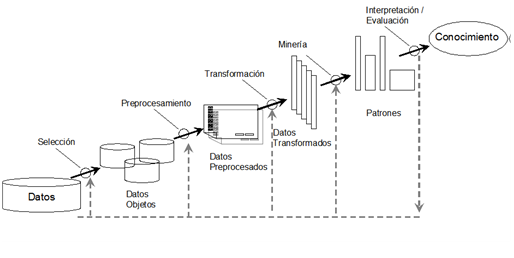
\includegraphics[scale=1]{images/kdd.png}
	\caption[Proceso KDD.]{Proceso KDD.}
	\label{fig:procesoKDD}
\end{figure}

\section{Herramientas}
\label{sec:herramientas}

	Esta sección busca dar a conocer al lector las herramientas de \textit{software} utilizadas para desarrollar el sistema propuesto.

	\subsection{Play Framework}
	\label{subsec:playframework}

	Es un \textit{framework} de código abierto para aplicaciones \textit{web} escrito en \textit{Java} y \textit{Scala}, el cual sigue el patrón de arquitectura \textit{Modelo-Vista-Controlador} (MVC). Utiliza el paradigma de diseño "Convención sobre configuración", el cual apunta a reducir la toma de decisiones que debe tomar el desarrollador sin perder flexibilidad. 

	Se enfoca en la productividad a aplicaciones \textit{RESTful}.

	Elimina la desventaja de desarrollo al utilizar \textit{Java} dada por el continuo ciclo de compilar-empaquetamiento-despliegue. Al detectar cambios en el código realiza inmediatamente la compilación y actualiza en la JVM sin necesidad de reiniciar el servidor.

	Play no utilizar sesiones en su funcionar, privilegiando el uso de almacenamiento \textit{offline} o el uso de peticiones \textit{Ajax} para resolver problemas del lado del cliente.

	\subsection{Apache Storm}
	\label{subsec:apacheStorm}

	Apache Storm es un sistema de computación en tiempo real de código abierto. Simplifica el problema de flujos (\textit{streams}), de datos sin que estos tengan fin.

	Es escalable, tolerante a fallos y garantiza que toda la información será procesada. Presenta \textit{Benchmarks} que señalan que por nodo es capaz de procesar más de un millón de tuplas por segundo.

	Se compone principalmente de dos partes. La primera es denominada \textit{Spout} y es la encargada de recoger el flujo de datos de entrada. La segunda es denominada \textit{Bolt} y es la encargada de la transformación o procesado de los datos.

	Oficialmente es representado como puede verse en la Figura \ref{fig:stormBeLike}. donde los \textit{Spouts} son representados simulando ser llaves de agua desde donde fluyen los datos al sistema y los \textit{Bolts} como rayos donde se procesa el flujo.

	\begin{figure}[H]
		\centering
		\captionsetup{justification=centering}
		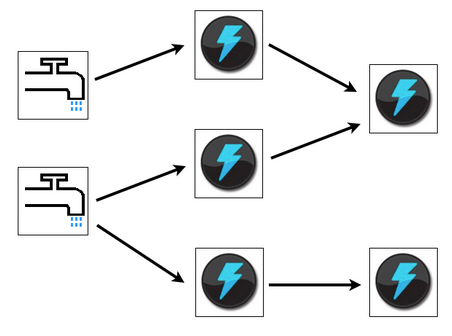
\includegraphics[scale=0.6]{images/stormBeLike.png}
		\caption[Representación del funcionamiento de Apache Storm.]{Representación del funcionamiento de Apache Storm.}
		\label{fig:stormBeLike}
	\end{figure}

	Uno de los puntos fuertes que tiene este sistema es que al crear una topología donde se instancian \textit{Bolts} y \textit{Spouts}, Storm se encarga de escalar el sistema distribuyendo los elementos en sus componentes.

	Al trabajar con \textit{Apache Storm}, como ya se ha descrito, se han de construir dos elementos: \textit{spout} y \textit{bolt}. Éstos elementos se construyen realizando heredando desde desde \textit{BaseRichSpout}, para el caso de \textit{spout} e implementando \textit{IRichBolt} para los \textit{bolt}. La descripción de los elementos de éstas clases se presentan en las secciones \ref{subsubsec:Spout} y \ref{subsubsec:Bolt}.

	\subsubsection{Spout}
	\label{subsubsec:Spout}

	\begin{figure}[H]
		\centering
		\captionsetup{justification=centering}
		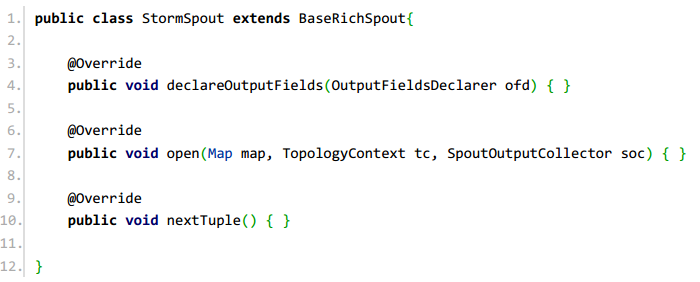
\includegraphics[scale=0.8]{images/SpoutBase.png}
		\caption[Construcción de un Spout.]{Construcción de un Spout.}
		\label{fig:spoutbase}
	\end{figure}

	En la figura \ref{fig:spoutbase} muestra la base para la implementación de un \textit{spout}. Cuenta con tres métodos:

	\begin{itemize}
	\item \textit{declareOutputFields}: declara nombres para las etiquetas que tendrá el objeto emitido.
	\item \textit{open}: Inicializa todos los elementos utilizados en el spout.
	\item \textit{nextTuple}: es llamado desde storm al recibir una nueva tupla para realizar una tarea.
	\end{itemize}	

	\subsubsection{Bolt}
	\label{subsubsec:Bolt}

	\begin{figure}[H]
		\centering
		\captionsetup{justification=centering}
		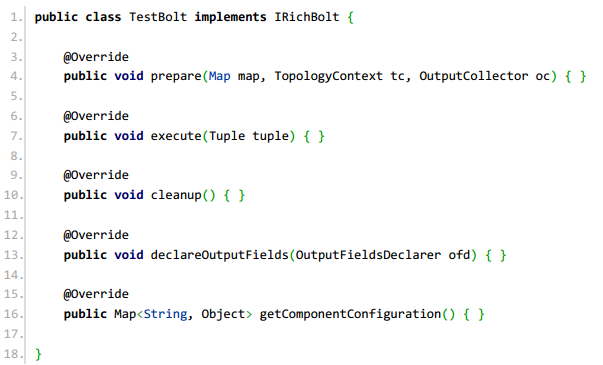
\includegraphics[scale=0.8]{images/BoltBase.png}
		\caption[Construcción de un Bolt.]{Construcción de un Bolt.}
		\label{fig:boltbase}
	\end{figure}

	La figura \ref{fig:boltbase} presenta la base para la implementación de un \textit{bolt}. Sus métodos se explican a continuación:

	\begin{itemize}
	\item \textit{prepare}: Similar al método \textit{open} para los \textit{spout}, realiza la misma función.
	\item \textit{execute}: Cumple la misma función que el método \textit{nextTuple}.
	\item \textit{cleanup}: Al finalizar una topología se llama este método para cerrar el \textit{bolt}.
	\item \textit{declareOutputFields}: declara nombres para las etiquetas que tendrá el objeto emitido.
	\item \textit{getComponentConfiguration}: Usado al querer cambiar una configuración del sistema.
	\end{itemize}

	\subsubsection{Topología}
	\label{subsubsec:topologia}

	Una topología de Storm es similar a un grafo. Cada nodo se encarga de procesar una determinada información y le pasa el testigo al siguiente nodo. Está compuesta por \textit{Spouts} y \textit{Bolts}. \cite{Storm}.

	\subsubsection{Cluster de Storm}
	\label{subsubsec:clusterStorm}

	Un cluster de Storm no muere, se queda siempre en espera de nuevos datos de entrada mientras el proceso siga activo.

	La arquitectura de Storm se divide en tres componentes:
	\begin{itemize}
	\item Master Node: Ejecuta el demonio llamado Nimbus, el cual es responsable de distribuir el código a través del cluster. Realiza la asignación y monitorización de tareas en las distintas máquinas del cluster.
	\item Worker Node: Ejecutan el demonio Supervisor, el cual se encarga de recoger y procesar los trabajos asignados en la máquina donde está corriendo. En caso de fallo de uno \textit{Worker Node}, Nimbus se dará cuenta y redirigirá el trabajo a otro.
	\item Zookeeper: Si bien no es un componente propio de Storm, es necesario para su funcionamiento, pues se encarga de coordinar Nimbus y Supervisor, además de mantener sus estados, pues ambos son \textit{stateless}.
	\end{itemize}

	\subsubsection{Modos de funcionamiento}
	\label{subsubsec:modoFuncionamientoStorm}

	Storm puede funcionar de dos modos: Local y Cluster. El primero es útil para el desarrollo, pues ejecuta toda la topología en una única JVM, por lo que pueden realizarse fácilmente pruebas de integración, depurar código, etcétera. Este modo simula, haciendo uso de \textit{Threads}, cada nodo del Cluster. \cite{Storm}.

	El modo Cluster es considerado el 'modo de producción' y es el modo donde el código es distribuido en máquinas diferentes dentro del Cluster.

	\subsubsection{Storm grouping}
	\label{subsubsec:StormGrouping}

	Se refiere a la forma en la que se van a compartir los datos entre los componentes. Como modelo de datos, Storm utiliza tuplas que son listas de valores con un nombre específico. El valor puede ser cualquier tipo, para ello se ha de implementar un serializador. \cite{Storm}.

	\begin{itemize}
	\item Shuffle grouping: Storm decide de forma \textit{round robin} la tarea a la que se va a enviar la tupla, de manera que la distribución sea equivalente entre todos los nodos.
	\item Fields gruoping: Se agrupan los \textit{streams} por un determinado campo de manera que se distribuyen los valores que cumplen una determinada condición a la misma tarea.
	\item All grouping: El \textit{stream} pasa por todas las tareas haciendo multicast.
	\item Grobal grouping: El \textit{stream} se envía al \textit{bolt} con ID más bajo.
	\item None grouping: Es un \textit{Shuffle grouping} donde el orden no es importante.
	\item Direct grouping: La tarea es la encargada de decidir hacia donde emitir especificando el ID del destinatario.
	\item Local grouping: Se utiliza el mismo \textit{bolt} si tiene una o más tareas en el mismo proceso.
	\end{itemize}

	\subsection{MongoDB}

	Base de datos no relacional (NoSQL) de código abierto escrita en C++ y está orientada al trabajo en documentos. Lo anterior quiere decir que, en lugar de guardar los datos en registros, lo hace en documentos y éstos son almacenada en una representación binaria de JSON conocida como BSON.

	Una de las diferencias fundamentales con respecto a las bases de datos relacionales es que no es necesario que se siga un esquema; en una misma colección - concepto similar a una tabla en las bases de datos relacionales - pueden tener distintos esquemas.

	MongoDB fue creado para brindar escalabilidad, rendimiento y disponibilidad. Puede ser utilizado en un servidor único como en múltiples. Esto se logra dado que MongoDB brinda un elevado rendimiento, tanto para lectura como para escritura, potenciando la computación en memoria.

	Las consultas en MongoDB se realizan como si se tratase de Javascript entregando como parámetro un objeto JSON. Por ejemplo, dado el documento presentado en la Figura ~\ref{fig:MongoJsonExample}, parte de una colección llamada 'Personas' en MongoDB:

	\begin{figure}[H]
		\centering
		\captionsetup{justification=centering}
		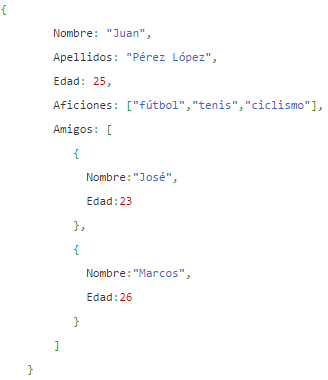
\includegraphics[scale=0.8]{images/MongoJsonExample.png}
		\caption[Documento en MongoDB.]{Documento en MongoDB.}
		\label{fig:MongoJsonExample}
	\end{figure}

	Una consulta para encontrar este elemento dentro de la colección se daría de la forma aprecida en la Figura ~\ref{fig:MongoJsonQueryExample}

	\begin{figure}[H]
		\centering
		\captionsetup{justification=centering}
		
\includegraphics[scale=0.8]{images/MongoJsonQueryExample.png}
		\caption[Consulta en MongoDB.]{Consulta en MongoDB.}
		\label{fig:MongoJsonQueryExample}
	\end{figure}

	En pruebas realizando operaciones habituales dentro de las bases de datos \cite{MongoPerformance} demostró que el tiempo de ejecución de MongoDB, como base de datos NoSQL, aventaja significativamente a las bases de datos relacionales más populares como lo son MySQL y PostgreSQL.


	
\chapter{Conclusiones}
\label{cap:conclusiones}
Lorem ipsum dolor sit cuchufl\'i barquillo bac\'an jote gamba listeilor po cahu\'in, luca mel\'on con vino pichanga coscacho ni ah\'i peinar la muñeca chuchada al chancho achoclonar. Chorrocientos pituto ubicatex huevo duro bolsero cachureo el hoyo del queque en cana huev\'on el año del loly hacerla corta impeque de miedo quilterry la raja longi ñecla. Hilo curado rayuela carrete quina guagua lorea piola ni ah\'i \citep{samza}.

% ### Bibliografía de la tesis ###
{\setstretch{1.0}						% Interlineado en las páginas finales
\bibliographystyle{apa-good}
\bibliography{bibliografia}
\addcontentsline{toc}{chapter}{Referencias bibliogr\'aficas} % Comando para agregar el índice a la Tabla de Contenido

% ### Optativo: Anexos de la tesis ###
\appendix
\addappheadtotoc							% Agregar Apéndice al índice. En caso de no poseer anexos, comentar
% ### Anexos ###
\chapter{Anexo de ejemplo}
\label{apendice:anexo1}

\textbf{Cómo obtener claves twitter}

\textbf{Glosario}


} % end \setstretch{1.0}

\end{document}
% end